\documentclass[12pt]{beamer}
\usepackage{lmodern}
%\usepackage[german]{babel}
\usepackage[utf8]{inputenc}
\usepackage[T1]{fontenc}
\usepackage[orientation=portrait,size=a0,scale=1.33]{beamerposter} % A0 = 84,1 x 118,9 cm (poster hanger 82 x 117, 10 mm margin => 2.5%)
\usepackage[margin=20mm,padding=20mm,blockspace=0.25\baselineskip]{beamerposterHSNR}
\usepackage{csquotes}
\usepackage{subcaption}
\usepackage
[
	backend=bibtex,
	hyperref=false,
	%style=alpha,
	%citestyle=alpha,
	doi=false,
	isbn=false,
	url=false,
	eprint=false,	
	sorting=nyt,
	giveninits=true
]
{biblatex}

%\addbibresource{bib/dice1945measures}
%\addbibresource{bib/frangi1998multiscale}

\title{Semantic Data Integration 2021 \\ Data Lake Team 2}
\author{\hspace{1em}{\vphantom{Wy}Supervised by Prof. Dr. Christoph Quix and Dr. Christoph Lange-Bever }} % you can underline the primary author



\affiliations{\hspace{1em}RWTH Aachen, Fraunhofer FIT}
\posterdate{01.\ April 2021 - 20.\ July 2021}
\posterconference{Semantic Data Lake}
\posterlocation{Aachen, Deutschland}


%


\posterlogotopleft{
\includegraphics[width=\textwidth]{cd/ipattern}}
\posterlogotopright{
\includegraphics[width=\textwidth]{cd/Signet_INF_2}}

\newcommand{\percent}{\raisebox{2pt}{\scalebox{0.825}{\%}}} % properly scaled percent-symbol

\begin{document}
%\usebackgroundtemplate{\includegraphics[width=\paperwidth]{hsnr_background}} % optional: background graphic
\begin{textblock}{0.5}(0.0, 0.0)

\begin{block}{Abstract}

\item Although big data has been discussed for some years, it still has many research challenges. It poses a huge difficulty to efficiently integrate, access, and query the large volume of diverse data in information silos with traditional ‘schema-on-write’ approaches such as data warehouses. Data lakes have been proposed as a solution to this problem as its vision is based on a generic and extensible architecture with a unified data model, facilitating the ingestion, storage and metadata management over heterogeneous data sources. The goal of this lab project was to further develop a prototype of a data lake system based on a four-layered architecture, where at the time the prototype was handed over, most of the functionality served the interaction and storage layer. The work of this group focused mostly on the interaction and transformation layer. The functionality was extended to incorporate the annotation of datasets with instances of an ontology to enrich stored data with additional metadata. In addition, a UI was added to process data graphically to build end-to-end data transformation pipelines.
\end{block}

\begin{block}{Introduction}

\item The variety of data poses a huge difficulty to efficiently integrate, access, and query the large volume of diverse data in information silos with traditional ‘schema-on-write’ approaches such as data warehouses. Data lakes have been proposed as a solution to this problem. "A data lake is a flexible, scalable data storage and management system, which ingests and stores raw data from heterogeneous sources in their original format, and provides query processing and data analytics in an on-the-fly manner." \cite{1}
\begin{figure}[H]
	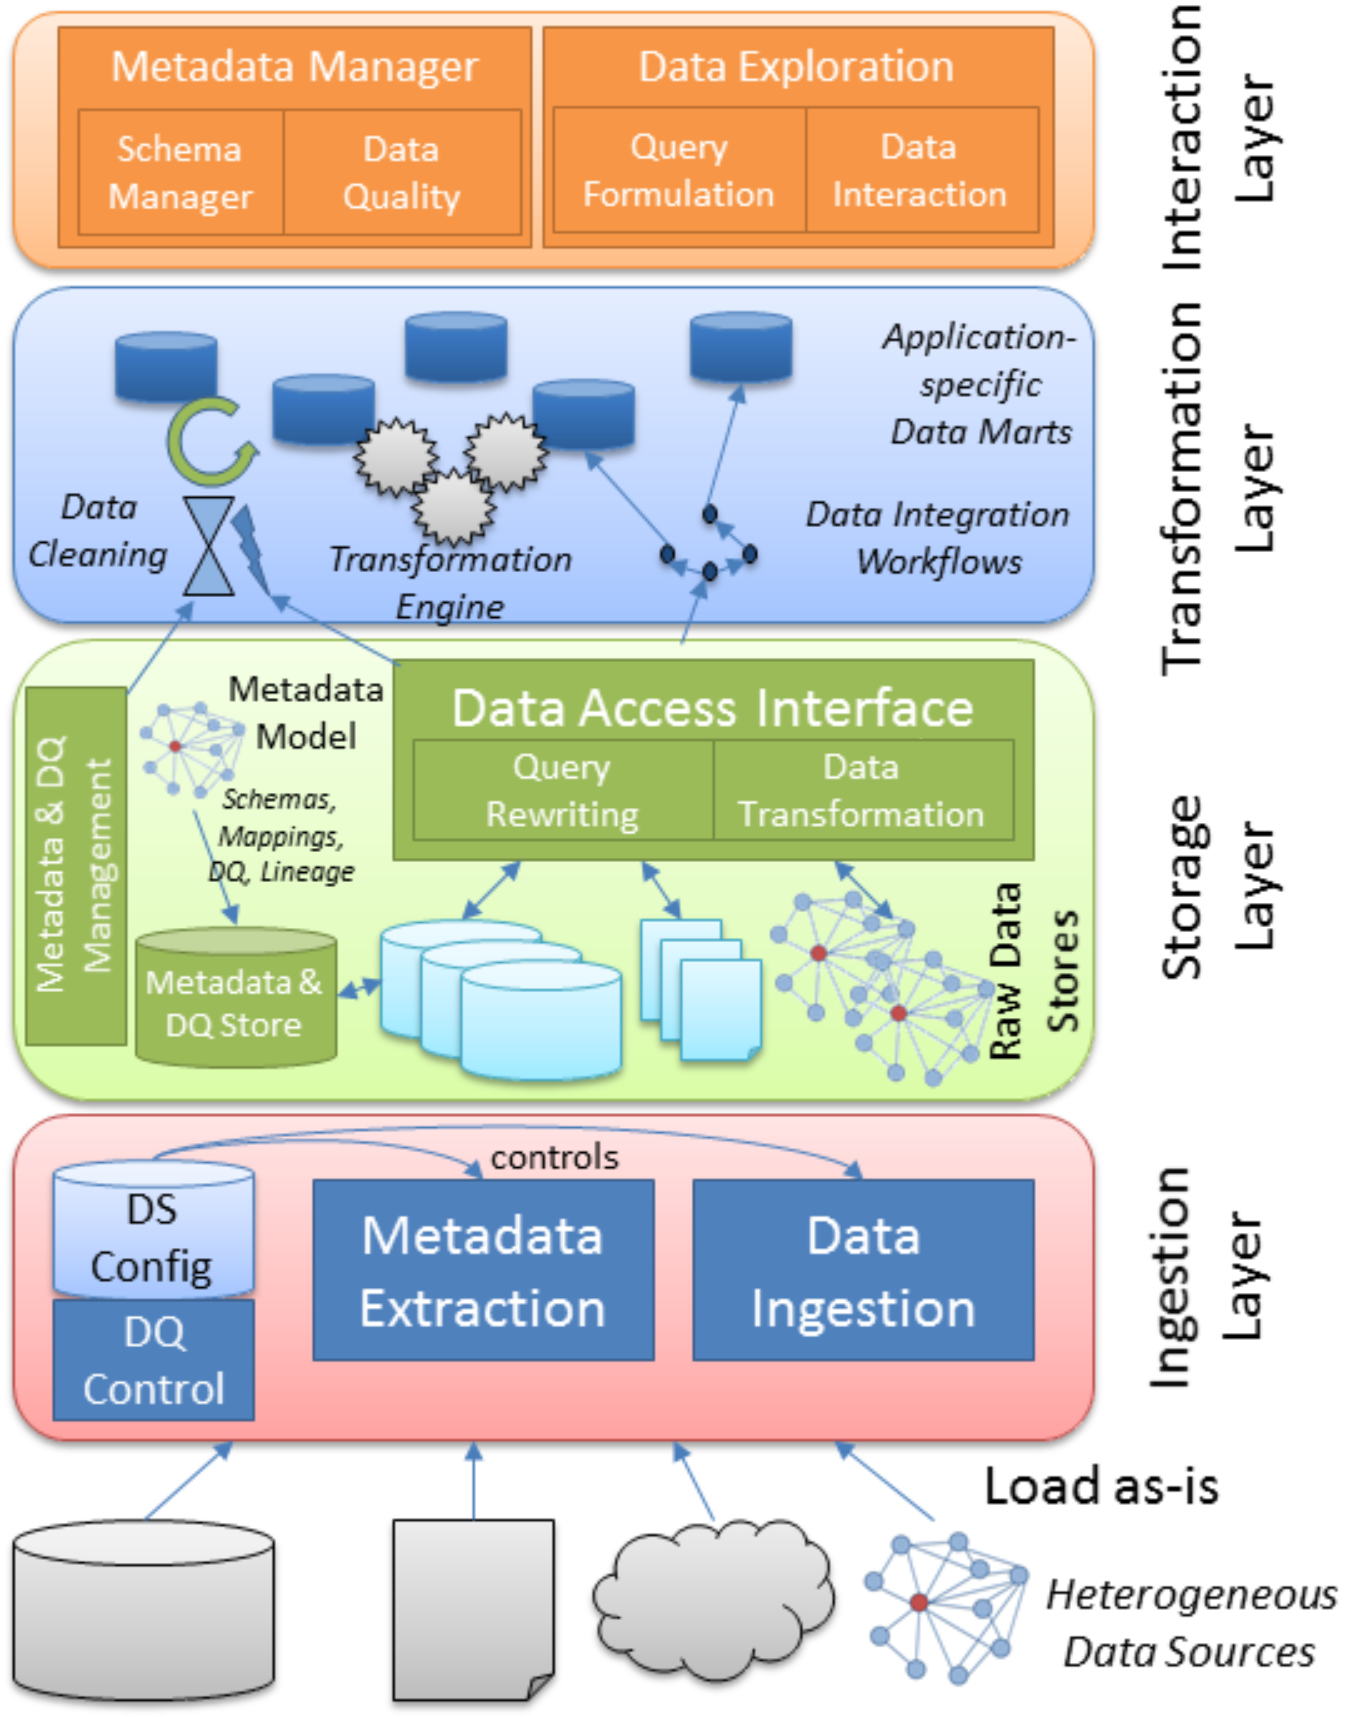
\includegraphics[width=0.7\linewidth]{data_lake_architecture.PNG}
	\caption{Data Lake Architecture with four layers \cite{2}} \label{Figure 1}
\end{figure}
For data reasoning, query processing, and data quality management and metadata management is crucial, because without any metadata, the data lake is hardly usable as the structure and semantics of the data are not known, which turns a data lake quickly into a ‘data swamp’. If sufficient metadata cannot be extracted from the sources automatically, a human expert has to provide additional information about the data source. \cite{1} One of the two major additions of this lab aimed to solve the aforementioned problem and established functionality to interlink datasets with instances of a user-defined ontology to enrich the available metadata For this Apache Jena-Fuseki is used as a triple-store. The second major addition is a Workflow diagram to enable the user to define end-to-end data transformation pipelines graphically. In the next section we list all of this labs additions to the project in order of importance, which can associated mostly to the interaction and transformation layer (see Figure 1).
\end{block}

\begin{block}{Added Functionality}
	\begin{enumerate}
	\item Add Semantic Information to Data
	\item New Frontend written with React and Material UI
	\item Graphical WorkFlow for Data Transformations written with ReactFlow
	\item Integrated Apache Zeppelin to the System
	\item Workspace Abstraction
	\item Datamart Deletion
	\item Complete refactoring of the projects code
	\item ER-Diagram and Backend Documentation using PyDocs
\end{enumerate}

\vspace{0.5\baselineskip}

\end{block}


\end{textblock}

%%%%%%% next page/column %%%%%%%%%%%%

\begin{textblock}{0.5}(0.5, 0.00)


\begin{block}{Architecture}
\begin{figure}[H]
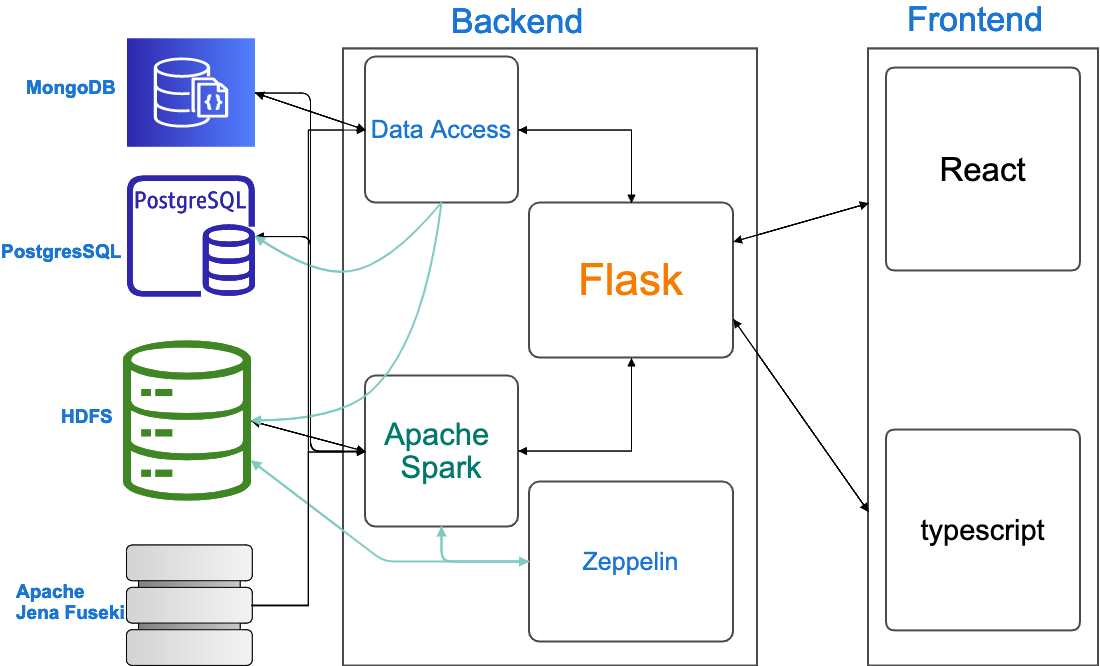
\includegraphics[width=0.8\linewidth,height=0.20\textheight]{data.png}
\caption{Architecture of the System. The left side displays databases and the underlying HDFS filesystem. The backend runs a Flask server with various data access function to store and process large-scale data using the Apache Spark analytics engine. The interaction between the frontend written in React is based on RESTful APIs. Figure created by Abdullah Zaid.} \label{Figure 1}
\end{figure} 
\end{block}




\begin{block}{Functionalities}
\begin{enumerate}
\item WorkFlow diagram enables the user to define Data Transformation pipelines which are executed upon data sources in a single Spark Session.
\begin{figure}[H]
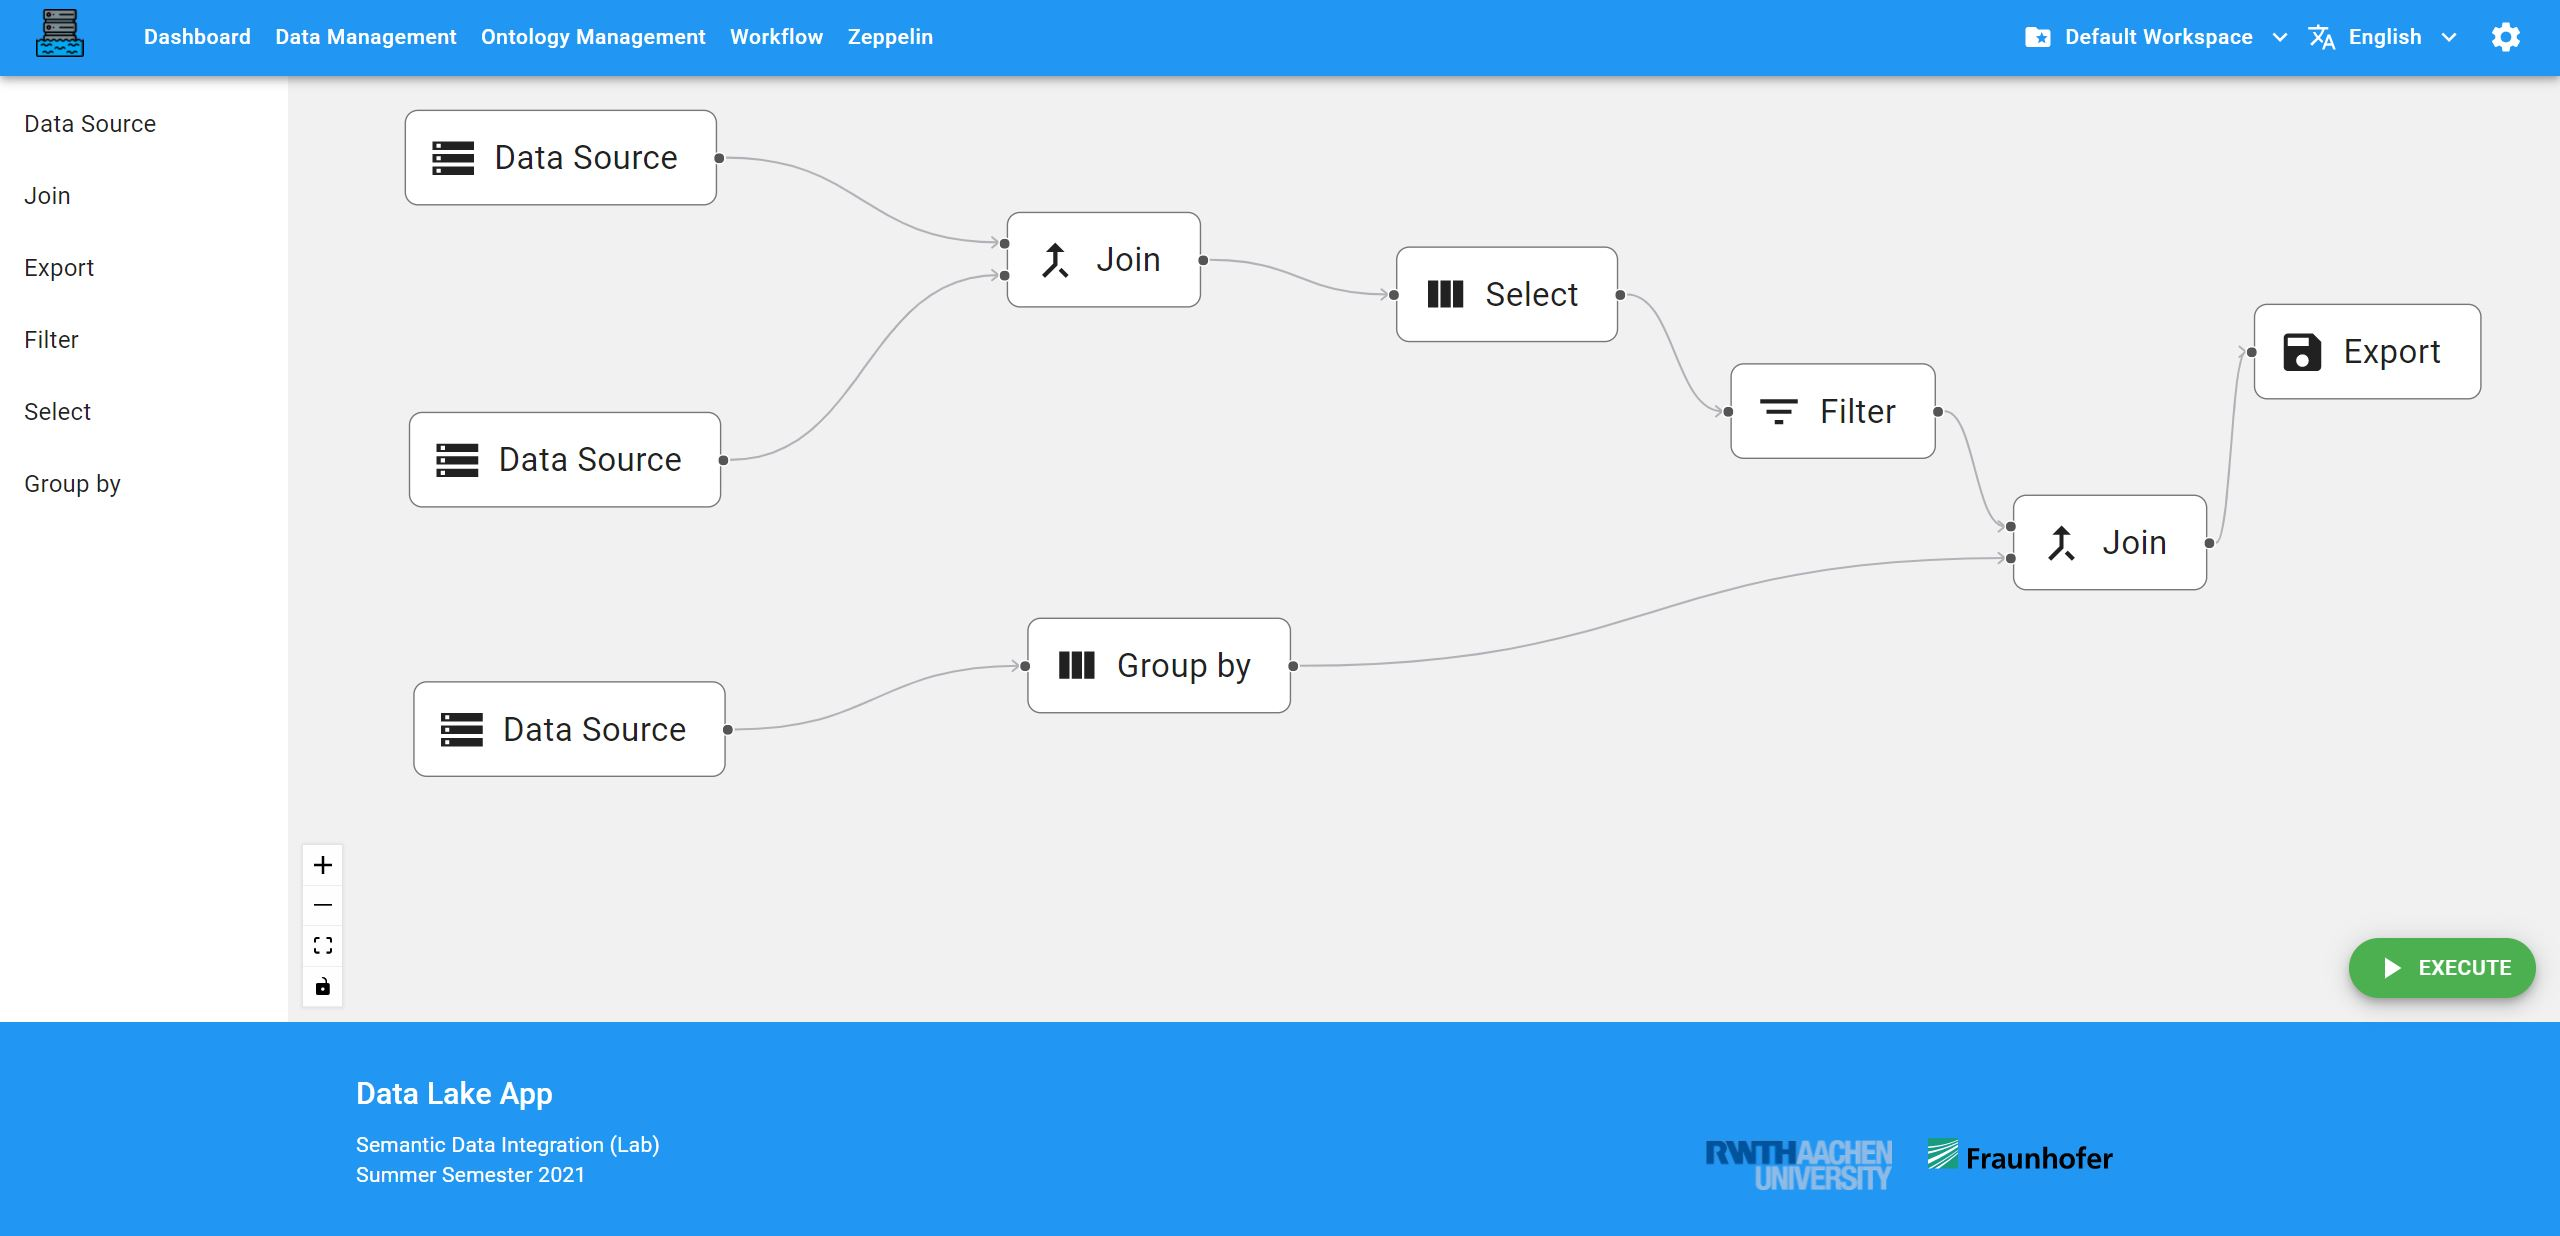
\includegraphics[width=1\linewidth]{datamart.JPG} 
\label{WorkFlow}
\end{figure}   
 
\item Datasets can be enriched by metadata using instances of user-defined ontologies. In the figure below the \textit{Date} column of a dataset is interlinked with an ontology instance with label \textit{primary key}.
\begin{figure}[H]
	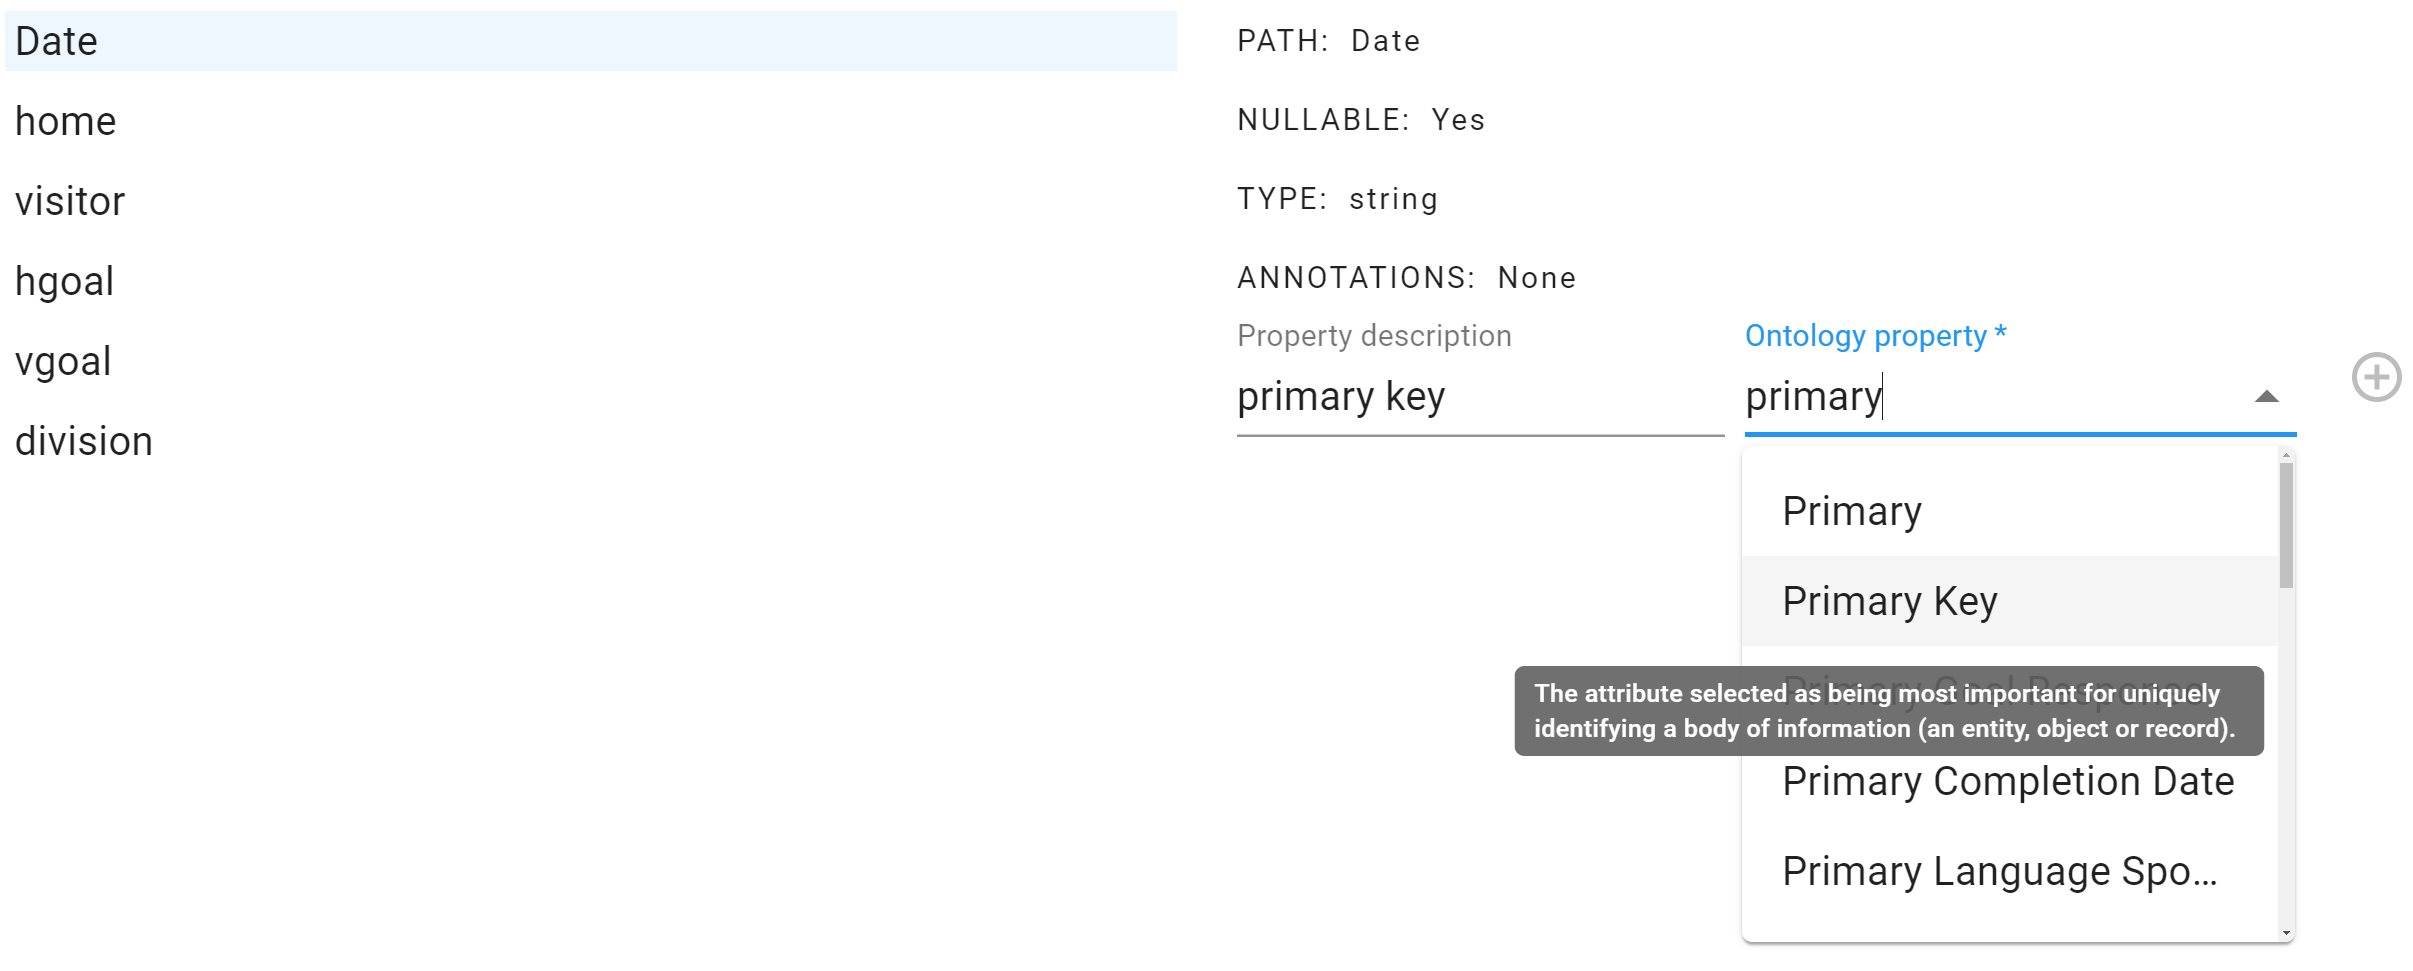
\includegraphics[width=0.9\linewidth]{annotation.PNG} 
	\label{WorkFlow}
\end{figure}   
    
\item Apache Zeppelin docker container is added to the system and the UI incorporate into the system's UI to perform data-driven,
interactive collaborative data analytics with pyspark.

\begin{figure}[H]
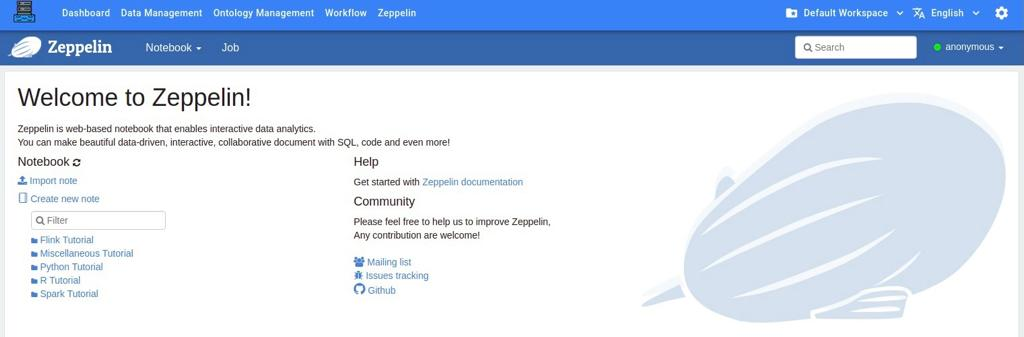
\includegraphics{zeppelin.jpeg}
\caption{Zeppelin} \label{Figure 1}
\end{figure} 
\end{enumerate}

\end{block}

% the bibliography
\vfill\vspace{7.5mm} % at the bottom, but at least some spacing
\begin{block}{References}
\item{[1] R. Hai, C. Quix, M. Jarke, "Data lake concept and systems: a survey"}
\item{[2] M. Jarke and C. Quix. “On warehouses, lakes, and spaces – the changing role of conceptual modeling for data integration.”}
\end{block}

\end{textblock}

\end{document}












%\colorbox{blue!45}{
%\begin{minipage}{\textwidth}
%\color{Blue} 
%The final line.
%\end{minipage}
%}